\documentclass{article}

\usepackage[letterpaper, margin=1in]{geometry}

\usepackage{titlesec}
%\usepackage[none]{hyphenat} % use only if there is a problem
% Use Unicode characters
\usepackage[utf8]{inputenc}

% tables
\usepackage{longtable,booktabs,array}
\usepackage{multirow}
\usepackage{afterpage}

% figures
\usepackage{wrapfig}
\usepackage{lscape}
\usepackage{rotating}
\usepackage{graphicx}
\graphicspath{assets}
\usepackage{times}
\usepackage{caption}
\usepackage{float}
\floatstyle{plaintop}
\restylefloat{table}

\title{Supplementary material for "Gut-resident microorganisms and their genes are associated with cognition and neuroanatomy in children"}

\begin{document}

\baselineskip24pt

\maketitle

\begin{figure}[h]
    \centering
    \includegraphics[width=0.9\textwidth]{assets/Supp_Figure1.png}
    \captionsetup{labelformat=empty}
    \caption{
        \textbf{Figure S1}: Sample collection by age - related to Figure 1A. A histogram showing the number of samples
        included in this study by the age of the child when the sample was collected.
    }
\end{figure}

\begin{figure}[h]
    \centering
    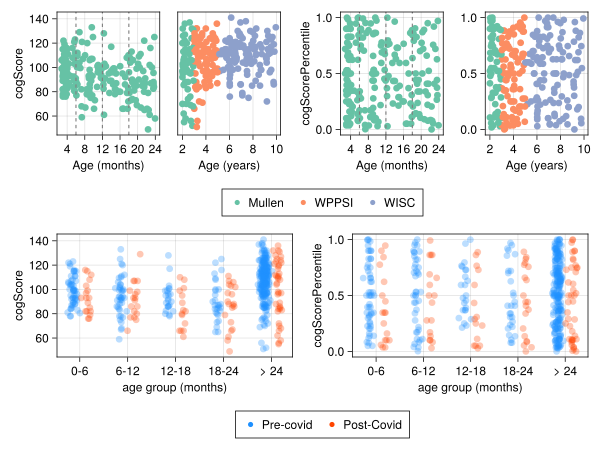
\includegraphics[width=0.9\textwidth]{assets/Supp_Figure2.png}
    \captionsetup{labelformat=empty}
    \caption{
        \textbf{Figure S2}: Principal coordinates analysis of taxonomic profiles - 
        related to Figure 1C. PCoAs are colored by the relative abundance per-sample
        of major phyla (Bacteroidetes, top left; Firmicutes, bottom left)
        and genera (\textit{Prevotella}, top right; \textit{Bifidobacterium}, bottom right).
    }
\end{figure}

\begin{figure}[h]
    \centering
    \includegraphics[width=0.9\textwidth]{assets/Supp_Figure3.png}
    \captionsetup{labelformat=empty}
    \caption{
        \textbf{Figure S3}: Cognitive assessment scores based on age
        and COVID-19. Scores in red were collected after March of 2020.
    }
\end{figure}

\begin{figure}[h]
  \centering
  \includegraphics[width=0.9\textwidth]{assets/Supp_Figure4.png}
  \captionsetup{labelformat=empty}
  \caption{
      \textbf{Figure S4}: Pareto plots for RFs of cognitive function - related to Figure 3C-D.
      The cumulative importance (orange line), as well as ranked importance (blue bars)
      of features (species) in models of cogntive performance score
      in children from birth to 6 months (top) or
      in children from 18 to 120 months (bottom).
  }
\end{figure}

\begin{figure}[h]
  \centering
  \includegraphics[width=0.9\textwidth]{assets/Supp_Figure5.png}
  \captionsetup{labelformat=empty}
  \caption{
      \textbf{Figure S5}: Heatmap of feature importances for each brain region -
      related to Figure 4B. This heatmap contains all features included in models
      (including age) and all brain segments. Importance values over 0.04
      are colored white.
  }
\end{figure}

\begin{sidewaysfigure}[h]
  \centering
  \includegraphics[width=0.9\textwidth]{assets/Supp_Figure6.png}
  \captionsetup{labelformat=empty}
  \caption{
      \textbf{Figure S6}: Species feature importances in brain region RFs - related to Figure 4C.
      All species (plus sex and maternal education) feature importances in each brain region model.
      X-axis is rank-ordered by median importance across all brain region models.
  }
\end{sidewaysfigure}

\begin{figure}[h]
  \centering
  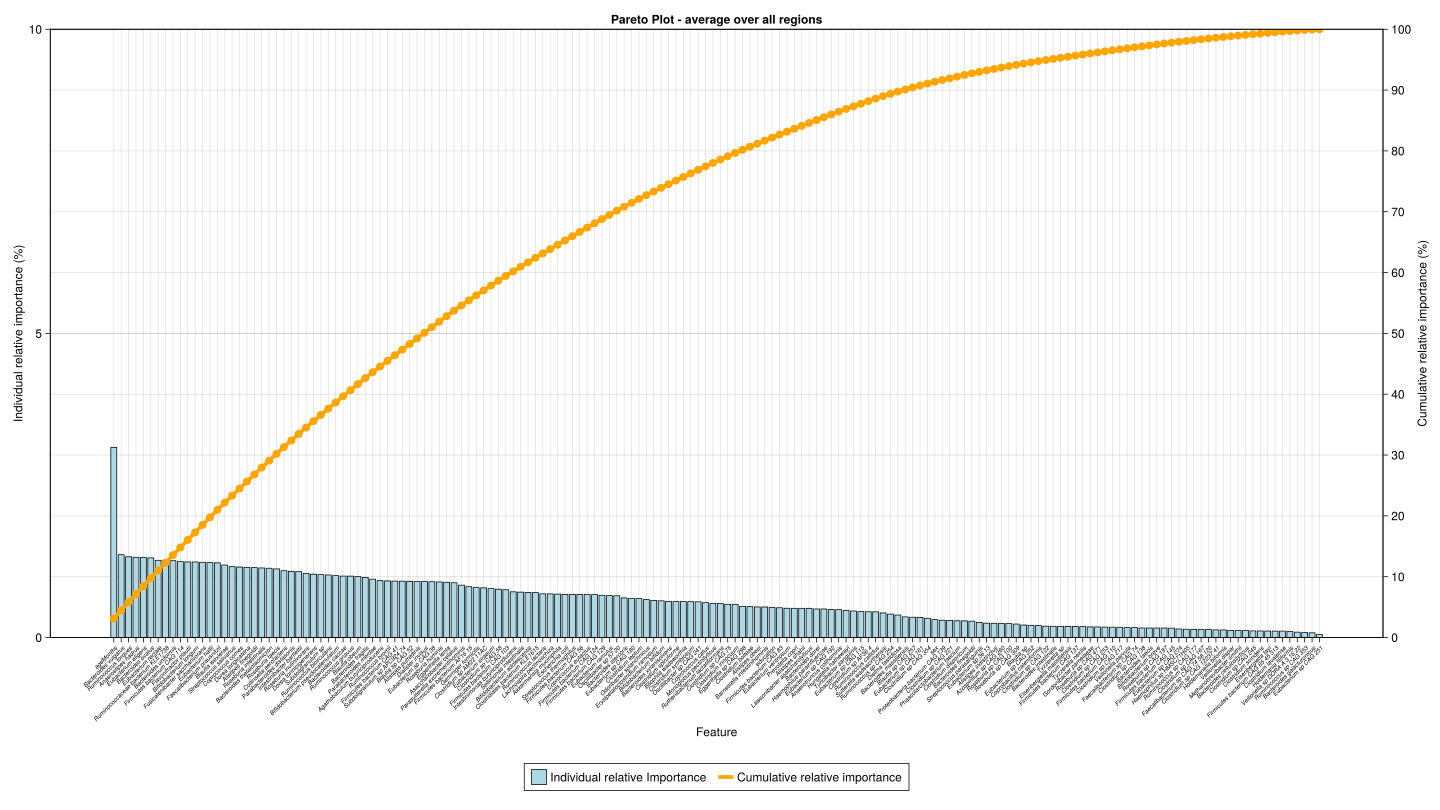
\includegraphics[width=0.9\textwidth]{assets/Supp_Figure7.png}
  \captionsetup{labelformat=empty}
  \caption{
      \textbf{Figure S7}: Pareto plots for RFs of cognitive function - related to Figure 4.
      The cumulative average importance (orange line), as well as ranked average importance (blue bars)
      of features (species) in models of brain region size.
  }
\end{figure}


\begin{table}[h]
    \begin{centering}
    \tiny
    \begin{tabular}{|r|r|r|r|r|}
      \hline\hline
      \textbf{Rank} & \textbf{Variable} & \textbf{Average fitness-weighted importance} & \textbf{Relative fitness-weighted importance} & \textbf{Rank-cumulative relative importance } \\\hline
      1 & \textit{Erysipelatoclostridium ramosum} & 0.00122 & 5.57 \% & 5.57 \% \\
      2 & \textit{ageMonths} & 0.00095 & 4.31 \% & 9.88 \% \\
      3 & \textit{Eggerthella lenta} & 0.00084 & 3.82 \% & 13.7 \% \\
      4 & \textit{Escherichia coli} & 0.00083 & 3.8 \% & 17.5 \% \\
      5 & \textit{Bifidobacterium longum} & 0.00077 & 3.51 \% & 21.01 \% \\
      6 & \textit{Veillonella parvula} & 0.00075 & 3.42 \% & 24.43 \% \\
      7 & \textit{Bifidobacterium breve} & 0.00072 & 3.26 \% & 27.68 \% \\
      8 & \textit{Klebsiella variicola} & 0.00065 & 2.98 \% & 30.66 \% \\
      9 & \textit{Enterococcus faecalis} & 0.00064 & 2.91 \% & 33.57 \% \\
      10 & \textit{Streptococcus salivarius} & 0.00062 & 2.84 \% & 36.42 \% \\
      11 & \textit{Klebsiella pneumoniae} & 0.00062 & 2.82 \% & 39.24 \% \\
      12 & \textit{Bifidobacterium bifidum} & 0.00057 & 2.59 \% & 41.83 \% \\
      13 & \textit{Flavonifractor plautii} & 0.00056 & 2.55 \% & 44.38 \% \\
      14 & \textit{Ruminococcus gnavus} & 0.00055 & 2.52 \% & 46.9 \% \\
      15 & \textit{Veillonella atypica} & 0.00053 & 2.41 \% & 49.31 \% \\
      16 & \textit{Klebsiella quasipneumoniae} & 0.0005 & 2.29 \% & 51.6 \% \\
      17 & \textit{Gordonibacter pamelaeae} & 0.00048 & 2.17 \% & 53.77 \% \\
      18 & \textit{Clostridioides difficile} & 0.00044 & 2.02 \% & 55.79 \% \\
      19 & \textit{Clostridium innocuum} & 0.00041 & 1.87 \% & 57.66 \% \\
      20 & \textit{Streptococcus parasanguinis} & 0.00038 & 1.73 \% & 59.38 \% \\
      21 & \textit{Blautia wexlerae} & 0.00036 & 1.65 \% & 61.03 \% \\
      22 & \textit{Bacteroides vulgatus} & 0.00036 & 1.65 \% & 62.68 \% \\
      23 & \textit{Clostridium neonatale} & 0.00033 & 1.51 \% & 64.19 \% \\
      24 & \textit{Enterococcus gallinarum} & 0.00031 & 1.4 \% & 65.59 \% \\
      25 & \textit{Veillonella dispar} & 0.00029 & 1.33 \% & 66.92 \% \\
      26 & \textit{Collinsella aerofaciens} & 0.00029 & 1.32 \% & 68.24 \% \\
      27 & \textit{Clostridium paraputrificum} & 0.00028 & 1.27 \% & 69.51 \% \\
      28 & \textit{Parabacteroides distasonis} & 0.00028 & 1.26 \% & 70.78 \% \\
      29 & \textit{Collinsella stercoris} & 0.00027 & 1.25 \% & 72.02 \% \\
      30 & \textit{Intestinibacter bartlettii} & 0.00027 & 1.22 \% & 73.25 \% \\
      31 & \textit{Bacteroides uniformis} & 0.00027 & 1.21 \% & 74.46 \% \\
      32 & \textit{Streptococcus mitis} & 0.00026 & 1.16 \% & 75.63 \% \\
      33 & \textit{Bacteroides ovatus} & 0.00024 & 1.1 \% & 76.73 \% \\
      34 & \textit{Klebsiella oxytoca} & 0.00024 & 1.1 \% & 77.82 \% \\
      35 & \textit{Hungatella hathewayi} & 0.00023 & 1.03 \% & 78.86 \% \\
      36 & \textit{Veillonella infantium} & 0.00022 & 0.98 \% & 79.84 \% \\
      37 & \textit{Clostridium sp 7 2 43FAA} & 0.00021 & 0.95 \% & 80.78 \% \\
      38 & \textit{Haemophilus parainfluenzae} & 0.00021 & 0.94 \% & 81.72 \% \\
      39 & \textit{Parabacteroides merdae} & 0.00019 & 0.88 \% & 82.6 \% \\
      40 & \textit{Clostridium bolteae} & 0.00018 & 0.83 \% & 83.43 \% \\
      41 & \textit{Clostridium perfringens} & 0.00018 & 0.83 \% & 84.26 \% \\
      42 & \textit{Bifidobacterium adolescentis} & 0.00018 & 0.82 \% & 85.07 \% \\
      43 & \textit{Bifidobacterium pseudocatenulatum} & 0.00016 & 0.75 \% & 85.82 \% \\
      44 & \textit{Enterococcus avium} & 0.00016 & 0.72 \% & 86.53 \% \\
      45 & \textit{Bacteroides thetaiotaomicron} & 0.00015 & 0.7 \% & 87.23 \% \\
      46 & \textit{Akkermansia muciniphila} & 0.00015 & 0.68 \% & 87.91 \% \\
      47 & \textit{Bacteroides caccae} & 0.00015 & 0.67 \% & 88.58 \% \\
      48 & \textit{Citrobacter youngae} & 0.00014 & 0.63 \% & 89.21 \% \\
      49 & \textit{Sellimonas intestinalis} & 0.00014 & 0.62 \% & 89.84 \% \\
      50 & \textit{Enterobacter cloacae complex} & 0.00013 & 0.6 \% & 90.44 \% \\
      51 & \textit{Streptococcus thermophilus} & 0.00013 & 0.6 \% & 91.04 \% \\
      52 & \textit{Lactobacillus rhamnosus} & 0.00013 & 0.58 \% & 91.62 \% \\
      53 & \textit{Bacteroides stercoris} & 0.00012 & 0.56 \% & 92.18 \% \\
      54 & \textit{Klebsiella michiganensis} & 0.00012 & 0.55 \% & 92.73 \% \\
      55 & \textit{Enterococcus faecium} & 0.0001 & 0.45 \% & 93.18 \% \\
      56 & \textit{Veillonella sp T11011 6} & 0.0001 & 0.43 \% & 93.61 \% \\
      57 & \textit{Streptococcus vestibularis} & 9.0e-5 & 0.43 \% & 94.04 \% \\
      58 & \textit{Ruthenibacterium lactatiformans} & 9.0e-5 & 0.42 \% & 94.45 \% \\
      59 & \textit{Bacteroides fragilis} & 9.0e-5 & 0.41 \% & 94.86 \% \\
      60 & \textit{Anaerostipes caccae} & 9.0e-5 & 0.4 \% & 95.25 \% \\
      61 & \textit{Enterococcus casseliflavus} & 9.0e-5 & 0.39 \% & 95.65 \% \\
      62 & \textit{Citrobacter freundii} & 8.0e-5 & 0.39 \% & 96.03 \% \\
      63 & \textit{Proteus mirabilis} & 8.0e-5 & 0.39 \% & 96.42 \% \\
      64 & \textit{Collinsella intestinalis} & 8.0e-5 & 0.37 \% & 96.8 \% \\
      65 & \textit{Varibaculum cambriense} & 8.0e-5 & 0.37 \% & 97.16 \% \\
      66 & \textit{Bilophila wadsworthia} & 7.0e-5 & 0.34 \% & 97.5 \% \\
      67 & \textit{Bifidobacterium scardovii} & 7.0e-5 & 0.3 \% & 97.8 \% \\
      68 & \textit{Aeriscardovia aeriphila} & 6.0e-5 & 0.29 \% & 98.1 \% \\
      69 & \textit{Morganella morganii} & 6.0e-5 & 0.26 \% & 98.36 \% \\
      70 & \textit{Bacteroides massiliensis} & 6.0e-5 & 0.25 \% & 98.61 \% \\
      71 & \textit{Clostridium symbiosum} & 5.0e-5 & 0.22 \% & 98.84 \% \\
      72 & \textit{Lactococcus lactis} & 5.0e-5 & 0.22 \% & 99.05 \% \\
      73 & \textit{Bacteroides dorei} & 4.0e-5 & 0.2 \% & 99.26 \% \\
      74 & \textit{Actinomyces sp HPA0247} & 4.0e-5 & 0.19 \% & 99.44 \% \\
      75 & \textit{Bacteroides xylanisolvens} & 3.0e-5 & 0.14 \% & 99.58 \% \\
      76 & \textit{Phascolarctobacterium faecium} & 3.0e-5 & 0.12 \% & 99.7 \% \\
      77 & \textit{Streptococcus pasteurianus} & 2.0e-5 & 0.11 \% & 99.8 \% \\
      78 & \textit{Fusicatenibacter saccharivorans} & 2.0e-5 & 0.1 \% & 99.91 \% \\
      79 & \textit{Ruminococcus torques} & 2.0e-5 & 0.09 \% & 100.0 \% \\\hline\hline
    \end{tabular}
    \caption*{
        \textbf{Table S1A}: Feature importances for RF models of cognitive performance
        based on taxonomic profiles in children under 6 months old.
    }
    \end{centering}
  \end{table}

\begin{table}[h]
  \begin{centering}
    \tiny
    \begin{tabular}{|r|r|r|r|r|}
      \hline\hline
      \textbf{Rank} & \textbf{Variable} & \textbf{Average fitness-weighted importance} & \textbf{Relative fitness-weighted importance} & \textbf{Rank-cumulative relative importance } \\\hline
      1 & \textit{ageMonths} & 0.02129 & 6.48 \% & 6.48 \% \\
      2 & \textit{Faecalibacterium prausnitzii} & 0.00859 & 2.61 \% & 9.09 \% \\
      3 & \textit{Bifidobacterium pseudocatenulatum} & 0.00598 & 1.82 \% & 10.91 \% \\
      4 & \textit{Asaccharobacter celatus} & 0.00586 & 1.78 \% & 12.7 \% \\
      5 & \textit{Eubacterium eligens} & 0.00536 & 1.63 \% & 14.33 \% \\
      6 & \textit{Bifidobacterium longum} & 0.00536 & 1.63 \% & 15.96 \% \\
      7 & \textit{Streptococcus parasanguinis} & 0.00517 & 1.57 \% & 17.53 \% \\
      8 & \textit{Ruminococcus gnavus} & 0.00507 & 1.54 \% & 19.08 \% \\
      9 & \textit{Roseburia faecis} & 0.00506 & 1.54 \% & 20.62 \% \\
      10 & \textit{Bacteroides vulgatus} & 0.00482 & 1.47 \% & 22.08 \% \\
      11 & \textit{Megamonas funiformis} & 0.00475 & 1.45 \% & 23.53 \% \\
      12 & \textit{Fusicatenibacter saccharivorans} & 0.00471 & 1.43 \% & 24.96 \% \\
      13 & \textit{Blautia wexlerae} & 0.00468 & 1.42 \% & 26.38 \% \\
      14 & \textit{Roseburia hominis} & 0.00464 & 1.41 \% & 27.79 \% \\
      15 & \textit{Eubacterium hallii} & 0.00462 & 1.41 \% & 29.2 \% \\
      16 & \textit{Parasutterella excrementihominis} & 0.0044 & 1.34 \% & 30.54 \% \\
      17 & \textit{Anaerostipes hadrus} & 0.00436 & 1.33 \% & 31.87 \% \\
      18 & \textit{Blautia obeum} & 0.00413 & 1.26 \% & 33.12 \% \\
      19 & \textit{Agathobaculum butyriciproducens} & 0.00395 & 1.2 \% & 34.32 \% \\
      20 & \textit{Haemophilus parainfluenzae} & 0.00386 & 1.18 \% & 35.5 \% \\
      21 & \textit{Gordonibacter pamelaeae} & 0.0038 & 1.16 \% & 36.66 \% \\
      22 & \textit{Alistipes finegoldii} & 0.00376 & 1.14 \% & 37.8 \% \\
      23 & \textit{Dorea longicatena} & 0.00373 & 1.14 \% & 38.94 \% \\
      24 & \textit{Flavonifractor plautii} & 0.00365 & 1.11 \% & 40.05 \% \\
      25 & \textit{Streptococcus salivarius} & 0.00362 & 1.1 \% & 41.15 \% \\
      26 & \textit{Adlercreutzia equolifaciens} & 0.00355 & 1.08 \% & 42.23 \% \\
      27 & \textit{Veillonella parvula} & 0.00355 & 1.08 \% & 43.31 \% \\
      28 & \textit{Intestinibacter bartlettii} & 0.0035 & 1.07 \% & 44.38 \% \\
      29 & \textit{Alistipes putredinis} & 0.00341 & 1.04 \% & 45.41 \% \\
      30 & \textit{Ruthenibacterium lactatiformans} & 0.00335 & 1.02 \% & 46.43 \% \\
      31 & \textit{Bacteroides ovatus} & 0.00331 & 1.01 \% & 47.44 \% \\
      32 & \textit{Bacteroides fragilis} & 0.00331 & 1.01 \% & 48.45 \% \\
      33 & \textit{Bacteroides uniformis} & 0.0033 & 1.0 \% & 49.45 \% \\
      34 & \textit{Eubacterium rectale} & 0.0032 & 0.97 \% & 50.43 \% \\
      35 & \textit{Roseburia inulinivorans} & 0.00307 & 0.94 \% & 51.36 \% \\
      36 & \textit{Streptococcus thermophilus} & 0.00306 & 0.93 \% & 52.29 \% \\
      37 & \textit{Roseburia intestinalis} & 0.00305 & 0.93 \% & 53.22 \% \\
      38 & \textit{Bacteroides caccae} & 0.00298 & 0.91 \% & 54.13 \% \\
      39 & \textit{Ruminococcus bicirculans} & 0.00296 & 0.9 \% & 55.03 \% \\
      40 & \textit{Parabacteroides distasonis} & 0.00289 & 0.88 \% & 55.91 \% \\
      41 & \textit{Ruminococcus torques} & 0.00287 & 0.87 \% & 56.78 \% \\
      42 & \textit{Clostridium symbiosum} & 0.00283 & 0.86 \% & 57.65 \% \\
      43 & \textit{Collinsella stercoris} & 0.00281 & 0.85 \% & 58.5 \% \\
      44 & \textit{Bifidobacterium bifidum} & 0.00278 & 0.85 \% & 59.35 \% \\
      45 & \textit{Collinsella aerofaciens} & 0.00278 & 0.85 \% & 60.19 \% \\
      46 & \textit{Ruminococcus bromii} & 0.00275 & 0.84 \% & 61.03 \% \\
      47 & \textit{Eubacterium sp CAG 38} & 0.00275 & 0.84 \% & 61.87 \% \\
      48 & \textit{Erysipelatoclostridium ramosum} & 0.0027 & 0.82 \% & 62.69 \% \\
      49 & \textit{Gemmiger formicilis} & 0.00266 & 0.81 \% & 63.5 \% \\
      50 & \textit{Eggerthella lenta} & 0.00261 & 0.79 \% & 64.29 \% \\
      51 & \textit{Dorea formicigenerans} & 0.00253 & 0.77 \% & 65.06 \% \\
      52 & \textit{Parabacteroides merdae} & 0.00247 & 0.75 \% & 65.81 \% \\
      53 & \textit{Odoribacter splanchnicus} & 0.00246 & 0.75 \% & 66.56 \% \\
      54 & \textit{Bacteroides thetaiotaomicron} & 0.00246 & 0.75 \% & 67.31 \% \\
      55 & \textit{Coprococcus eutactus} & 0.00246 & 0.75 \% & 68.06 \% \\
      56 & \textit{Coprococcus comes} & 0.00245 & 0.74 \% & 68.8 \% \\
      57 & \textit{Tyzzerella nexilis} & 0.00241 & 0.73 \% & 69.54 \% \\
      58 & \textit{Megamonas hypermegale} & 0.00236 & 0.72 \% & 70.25 \% \\
      59 & \textit{Ruminococcus lactaris} & 0.00236 & 0.72 \% & 70.97 \% \\
      60 & \textit{Eubacterium siraeum} & 0.00234 & 0.71 \% & 71.69 \% \\
      61 & \textit{Clostridium sp CAG 58} & 0.00227 & 0.69 \% & 72.38 \% \\
      62 & \textit{Clostridium spiroforme} & 0.00225 & 0.69 \% & 73.06 \% \\
      63 & \textit{Veillonella atypica} & 0.00219 & 0.67 \% & 73.73 \% \\
      64 & \textit{Bifidobacterium adolescentis} & 0.00214 & 0.65 \% & 74.38 \% \\
      65 & \textit{Monoglobus pectinilyticus} & 0.00212 & 0.64 \% & 75.03 \% \\
      66 & \textit{Alistipes shahii} & 0.0021 & 0.64 \% & 75.67 \% \\
      67 & \textit{Eubacterium ramulus} & 0.0021 & 0.64 \% & 76.31 \% \\
      68 & \textit{Prevotella copri} & 0.00209 & 0.64 \% & 76.94 \% \\
      69 & \textit{Bacteroides xylanisolvens} & 0.00202 & 0.62 \% & 77.56 \% \\
      70 & \textit{Oscillibacter sp 57 20} & 0.00201 & 0.61 \% & 78.17 \% \\
      71 & \textit{Blautia sp CAG 257} & 0.00198 & 0.6 \% & 78.77 \% \\
      72 & \textit{Sutterella parvirubra} & 0.00198 & 0.6 \% & 79.38 \% \\
      73 & \textit{Akkermansia muciniphila} & 0.00192 & 0.58 \% & 79.96 \% \\
      74 & \textit{Clostridium bolteae} & 0.00186 & 0.57 \% & 80.53 \% \\
      75 & \textit{Clostridium leptum} & 0.00185 & 0.56 \% & 81.09 \% \\
      76 & \textit{Lachnospira pectinoschiza} & 0.00185 & 0.56 \% & 81.66 \% \\
      77 & \textit{Bacteroides stercoris} & 0.00185 & 0.56 \% & 82.22 \% \\
      78 & \textit{Clostridium innocuum} & 0.00184 & 0.56 \% & 82.78 \% \\
      79 & \textit{Escherichia coli} & 0.00183 & 0.56 \% & 83.33 \% \\
      80 & \textit{Eubacterium sp CAG 180} & 0.00179 & 0.55 \% & 83.88 \% \\
      81 & \textit{Intestinimonas butyriciproducens} & 0.00179 & 0.55 \% & 84.42 \% \\
      82 & \textit{Dialister invisus} & 0.00177 & 0.54 \% & 84.96 \% \\
      83 & \textit{Anaerotruncus colihominis} & 0.00171 & 0.52 \% & 85.48 \% \\
      84 & \textit{Bifidobacterium breve} & 0.00168 & 0.51 \% & 85.99 \% \\
      85 & \textit{Sellimonas intestinalis} & 0.00166 & 0.51 \% & 86.5 \% \\
      86 & \textit{Veillonella infantium} & 0.00162 & 0.49 \% & 86.99 \% \\
      87 & \textit{Bacteroides dorei} & 0.00161 & 0.49 \% & 87.48 \% \\
      88 & \textit{Proteobacteria bacterium CAG 139} & 0.0016 & 0.49 \% & 87.97 \% \\
      89 & \textit{Megamonas funiformis CAG 377} & 0.00152 & 0.46 \% & 88.43 \% \\
      90 & \textit{Bilophila wadsworthia} & 0.00152 & 0.46 \% & 88.89 \% \\
      91 & \textit{Hungatella hathewayi} & 0.00145 & 0.44 \% & 89.33 \% \\
      92 & \textit{Veillonella dispar} & 0.00144 & 0.44 \% & 89.77 \% \\
      93 & \textit{Turicimonas muris} & 0.00141 & 0.43 \% & 90.2 \% \\
      94 & \textit{Roseburia sp CAG 471} & 0.00141 & 0.43 \% & 90.63 \% \\
      95 & \textit{Eisenbergiella massiliensis} & 0.00137 & 0.42 \% & 91.05 \% \\
      96 & \textit{Firmicutes bacterium CAG 83} & 0.00127 & 0.39 \% & 91.44 \% \\
      97 & \textit{Barnesiella intestinihominis} & 0.00126 & 0.38 \% & 91.82 \% \\
      98 & \textit{Turicibacter sanguinis} & 0.00122 & 0.37 \% & 92.19 \% \\
      99 & \textit{Bifidobacterium catenulatum} & 0.00117 & 0.36 \% & 92.55 \% \\
      100 & \textit{Bacteroides finegoldii} & 0.00115 & 0.35 \% & 92.9 \% \\
      100+ & See Table file & ... & ... & ... \\\hline\hline
    \end{tabular}
    \caption*{
        \textbf{Table S1B}: Feature importances for RF models of cognitive performance
        based on taxonomic profiles in children over 18 months old.
    }
    \end{centering}
  \end{table}

  \begin{table}[h]
  
  \begin{centering}
    \tiny
    \begin{tabular}{|r|r|r|}
      \hline\hline
      \textbf{Segment} & \textbf{Mean absolute proportional error (MAPE)} & \textbf{Correlation coefficient (R)} \\\hline
      Left temporal & 0.0405 & 0.1278 \\
      Right temporal & 0.0393 & 0.0683 \\
      Left orbitofrontal & 0.0554 & 0.1862 \\
      Right orbitofrontal & 0.0614 & 0.1325 \\
      Left parietal & 0.0352 & 0.1767 \\
      Right parietal & 0.0451 & -0.1471 \\
      Left middle frontal & 0.0521 & -0.0002 \\
      Right middle frontal & 0.0385 & 0.0829 \\
      Left anterior cingulate & 0.0685 & 0.0917 \\
      Right anterior cingulate & 0.0739 & 0.2447 \\
      Left lateral occipital & 0.0622 & 0.2237 \\
      Right lateral occipital & 0.0544 & 0.2208 \\
      Left cerebellum white matter & 0.0667 & 0.4132 \\
      Right cerebellum white matter & 0.0698 & 0.4344 \\
      Left thalamus proper & 0.0534 & 0.1696 \\
      Right thalamus proper & 0.0499 & 0.1616 \\
      Left caudate & 0.099 & 0.0287 \\
      Right caudate & 0.083 & -0.01 \\
      Left putamen & 0.0592 & 0.1541 \\
      Right putamen & 0.0658 & 0.0107 \\
      Left pallidum & 0.0641 & 0.2967 \\
      Right pallidum & 0.0613 & 0.2644 \\
      Left hippocampus & 0.0541 & 0.0749 \\
      Right hippocampus & 0.0593 & -0.0937 \\
      Left amygdala & 0.0632 & 0.2879 \\
      Right amygdala & 0.0704 & 0.1787 \\
      Left accumbens area & 0.0941 & 0.2877 \\
      Right accumbens area & 0.1024 & -0.0406 \\
      Left basal forebrain & 0.2059 & 0.1544 \\
      Right basal forebrain & 0.1169 & 0.1234 \\
      Left cuneus & 0.0816 & 0.2345 \\
      Right cuneus & 0.075 & 0.0647 \\
      Left entorhinal & 0.0798 & 0.1904 \\
      Right entorhinal & 0.0822 & 0.0993 \\
      Left fusiform & 0.0572 & 0.3331 \\
      Right fusiform & 0.053 & 0.2482 \\
      Left isthmus cingulate & 0.0774 & -0.0409 \\
      Right isthmus cingulate & 0.0854 & 0.0735 \\
      Left lingual & 0.0688 & 0.4212 \\
      Right lingual & 0.0719 & 0.4336 \\
      Left parahippocampal & 0.0576 & 0.1535 \\
      Right parahippocampal & 0.0602 & 0.1341 \\
      Left paracentral & 0.0781 & 0.1309 \\
      Right paracentral & 0.084 & 0.0231 \\
      Left pars opercularis & 0.057 & 0.1464 \\
      Right pars opercularis & 0.0595 & 0.0301 \\
      Left pars orbitalis & 0.0821 & 0.0032 \\
      Right pars orbitalis & 0.1118 & 0.0235 \\
      Left pars triangularis & 0.0633 & 0.1743 \\
      Right pars triangularis & 0.0762 & 0.0434 \\
      Left pericalcarine & 0.1105 & 0.1997 \\
      Right pericalcarine & 0.0885 & 0.2729 \\
      Left postcentral & 0.0516 & 0.1681 \\
      Right postcentral & 0.0595 & 0.1349 \\
      Left posterior cingulate & 0.1338 & 0.1365 \\
      Right posterior cingulate & 0.1394 & 0.0628 \\
      Left precentral & 0.0654 & 0.2478 \\
      Right precentral & 0.0463 & 0.0656 \\
      Left precuneus & 0.0561 & 0.1443 \\
      Right precuneus & 0.0685 & 0.1499 \\
      Left superior frontal & 0.0398 & 0.1008 \\
      Right superior frontal & 0.0436 & -0.0961 \\
      Left supramarginal & 0.0668 & 0.0611 \\
      Right supramarginal & 0.0682 & -0.0008 \\
      Left insula & 0.0571 & -0.119 \\
      Right insula & 0.0562 & 0.0771 \\
      Cerebellar vermal lobules I V & 0.0846 & 0.1562 \\
      Cerebellar vermal lobules VI VII & 0.0813 & 0.006 \\
      Cerebellar vermal lobules VIII X & 0.0825 & 0.0781 \\
      Brain stem & 0.0766 & 0.6047 \\
      CSF & 0.1624 & 0.0713 \\\hline\hline
    \end{tabular}
    \caption*{
        \textbf{Table S2}: RF model performances predicting cortical and
        subcortical brain regions.
    }
    \end{centering}
  \end{table}


\begin{table}[h]
  \begin{centering}
    \begin{tabular}{|r|r|r|r|}
      \hline\hline
      \textbf{Input set} & \textbf{Age bracket} & \textbf{Microbiome encoding type} & \textbf{Demographics Provided? (sex, education)} \\\hline
      1 & \multirow{5}{*}{0 to 6 months} & Not provided & yes \\ \cline{3-4}
      2 &  & \multirow{2}{*}{Taxonomic profile} & no \\ \cline{4-4}
      3 &  &  & yes \\ \cline{3-4}
      4 &  & \multirow{2}{*}{Functional Profile (ECs)} & no \\ \cline{4-4}
      5 &  &  & yes \\ \cline{2-4}
      6 & \multirow{5}{*}{18 to 120 months} & Not provided & yes \\ \cline{3-4}
      7 &  & \multirow{2}{*}{Taxonomic profile} & no \\ \cline{4-4}
      8 &  &  & yes \\ \cline{3-4}
      9 &  & \multirow{2}{*}{Functional Profile (ECs)} & no \\ \cline{4-4}
      10 &  &  & yes \\\hline\hline
    \end{tabular}
    \caption*{
      \textbf{Table S3}: Experimental design and input composition for Random
      Forest experiments.
    }
  \end{centering}
\end{table}

\end{document}